\section{Results}

In this section, we present the results obtained throughout the development of the work, detailing the different approaches and techniques applied for image classification in the Intel Image Classification dataset.

Initially, we used a basic convolutional neural network (CNN), as presented in class, to establish an initial baseline. Next, we introduced the data augmentation technique to increase the diversity of the dataset and improve the model's performance, conducting training for 10 epochs.

Subsequently, we explored feedforward neural networks (FNNs), testing different combinations of hyperparameters. We continued the experiment by applying another CNN, again varying its hyperparameters. Both FNN and CNNs were trained for 30 epochs using data augmentation techniques.

Finally, we implemented the DenseNet architecture, a state-of-the-art network, and performed two experiments: one without data augmentation and another using the technique to analyze the impacts of this approach on an advanced model, conducting training for 30 epochs.

\subsection{CNN Model Class}

The first version of our Convolutional Neural Network (CNN) was designed with a straightforward architecture aimed at establishing a baseline performance metric. The model includes three convolutional layers, each followed by a max-pooling layer, with a fully connected dense layer and a dropout layer for regularization before the output layer. The specific architecture is as follows:

\begin{table}[H]
\centering
\caption{Architecture of the CNN Model}
\begin{tabular}{|l|c|c|}
\hline
\textbf{Layer (Type)}          & \textbf{Output Shape} & \textbf{Parameters} \\ \hline
Conv2D                         & (None, 148, 148, 32)  & 896                 \\ \hline
MaxPooling2D                   & (None, 74, 74, 32)    & 0                   \\ \hline
Conv2D                         & (None, 72, 72, 64)    & 18,496              \\ \hline
MaxPooling2D                   & (None, 36, 36, 64)    & 0                   \\ \hline
Conv2D                         & (None, 34, 34, 128)   & 73,856              \\ \hline
MaxPooling2D                   & (None, 17, 17, 128)   & 0                   \\ \hline
Flatten                        & (None, 36992)         & 0                   \\ \hline
Dense                          & (None, 128)           & 4,735,104           \\ \hline
Dropout                        & (None, 128)           & 0                   \\ \hline
Dense                          & (None, 6)           & 774           \\ \hline
\hline
\textbf{Total params:}        & \multicolumn{2}{l|}{4,829,126}              \\ \hline
\textbf{Trainable params:}    & \multicolumn{2}{l|}{4,829,126}              \\ \hline
\textbf{Non-trainable params:} & \multicolumn{2}{l|}{0}                      \\ \hline
\end{tabular}
\label{tab:cnn_architecture}
\end{table}


The model was compiled using the Adam optimizer with a default learning rate of 0.001. The Adam optimizer is well suited for this task due to its adaptive learning rate capabilities.
The loss function used is ”categorical crossentropy”, which is appropriate for multiclass classification problems, and the performance metric tracked during training was accuracy.
The performance of the first CNN was evaluated using training, validation, and test datasets. The model demonstrated a high accuracy on the training data but showed a significant drop in accuracy on the validation and test data, indicating potential overfitting.

The next figure provides a visual representation of the accuracy and loss trends for both training and validation data across the \textbf{10 epochs}, offering insights into the model's learning dynamics.
The model achieved higher accuracy on the training data compared to the validation and test data. This discrepancy suggests potential overfitting, where the model performs well on the data it has seen but struggles to generalize effectively to unseen data. This behavior is further corroborated by the loss values recorded during training and validation, which highlight the challenges in maintaining consistency across the dataset.

\begin{figure}[h!]
    \centering
    \begin{subfigure}[t]{0.45\textwidth} % Tamanho de cada subfigura
        \centering
        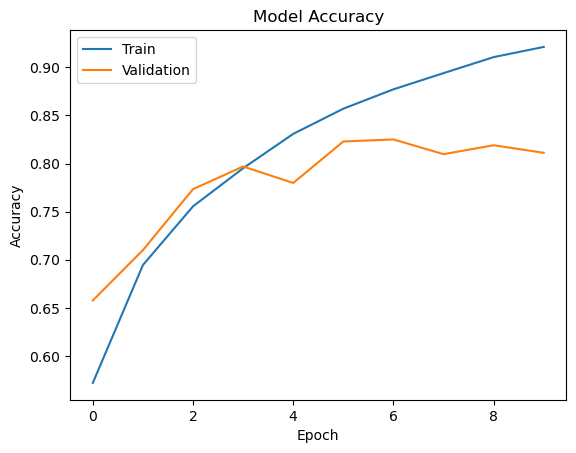
\includegraphics[width=\textwidth]{images/model_class_accuracy.png}
        \caption{Train vs Validation Accuracy}
        \label{fig:subfig1}
    \end{subfigure}
    \hfill
    \begin{subfigure}[t]{0.45\textwidth}
        \centering
        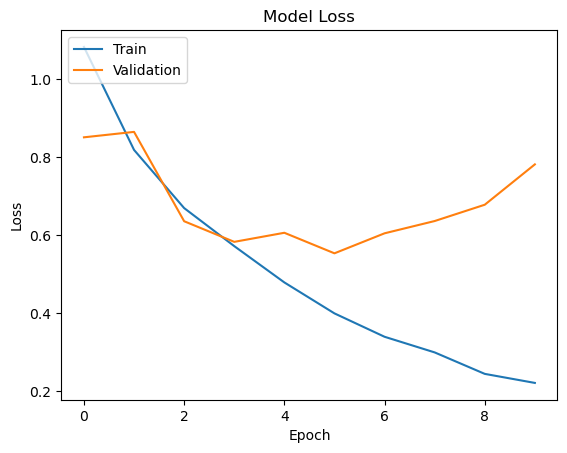
\includegraphics[width=\textwidth]{images/model_class_loss.png}
        \caption{Train vs Validation Loss}
        \label{fig:subfig2}
    \end{subfigure}
    \caption{Accuracy and Loss for the First Model}
    \label{fig:images}
\end{figure}

The graphs reveal that while the training accuracy consistently improves and the training loss decreases, the validation accuracy stagnates after the initial epochs, and the validation loss increases. This pattern further reinforces the indication of overfitting.

To gain a deeper understanding of the model's performance, we generated the confusion matrix for the test data and calculated the precision, recall, and F1-score, providing a more comprehensive evaluation of the model's effectiveness across different classes.

\begin{figure}[H]
    \centering
    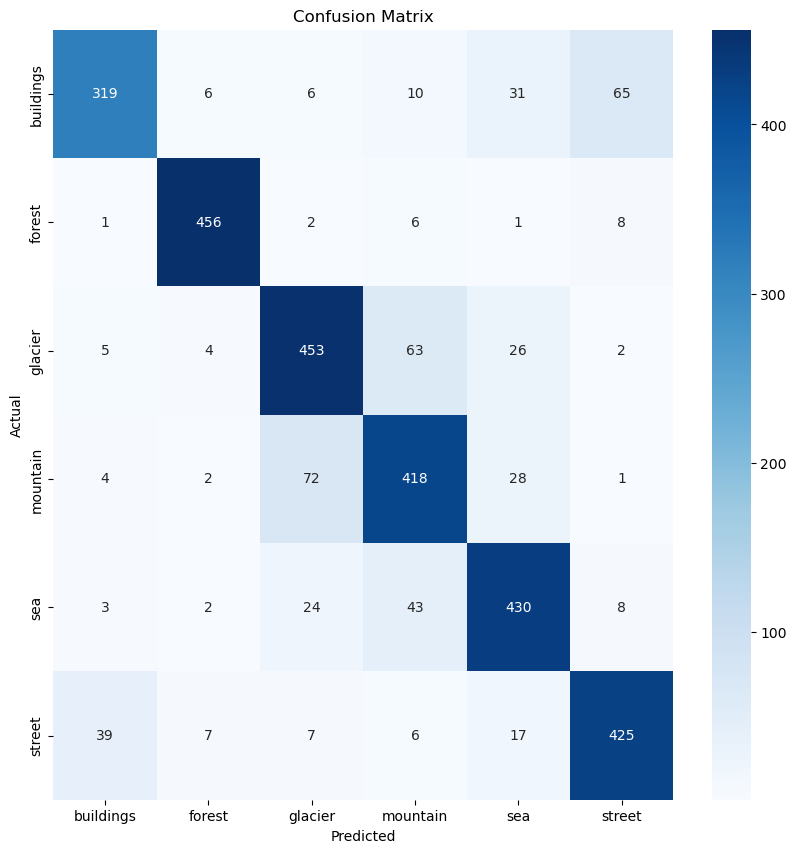
\includegraphics[width=1\linewidth]{images/model_aulas_confusion.png}
    \caption{Model Confusion Matrix}
    \label{fig:enter-label}
\end{figure}

\begin{figure}[H]
    \centering
    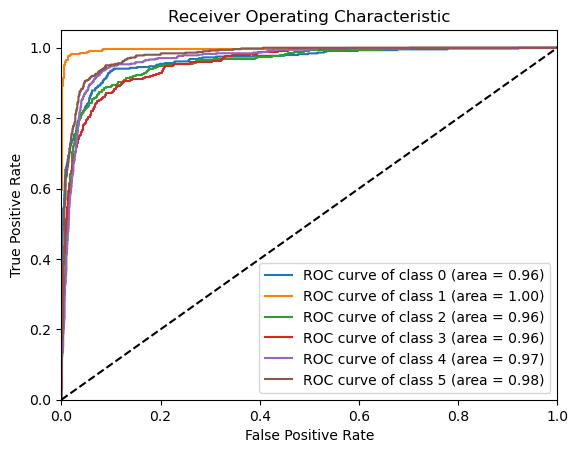
\includegraphics[width=1\linewidth]{images/modelo_aula_roc.png}
    \caption{Roc Curve}
    \label{fig:rocincial}
\end{figure}

\begin{table}[H]
    \centering
    \caption{Model Test Evaluation Metrics} 
    \begin{tabular}{||c|c|c|c|c||} 
        \hline
        Accuracy & F1 Score & Recall & Precision \\
        \hline\hline
        0.834 & 0.834 & 0.834 & 0.835 \\
        \hline
    \end{tabular}
    \label{tab:tab_LogReg}
\end{table}

Forests (1) are classified very accurately, with the majority of predictions falling in the correct category. Meanwhile, Buildings (0) are often misclassified as Streets (5), with 65 misclassifications, and Streets (5) are sometimes confused with Buildings (0) and Sea (4). On the same note, Mountains (3) and Glaciers (2) frequently get confused with each other, reflecting their visual similarities (72 mountains as glaciers and 63 glaciers as mountains).

The ROC (Receiver Operating Characteristic) curves for the six scene classes provide an overall view of the model’s ability to distinguish between different types of scenery. Each ROC curve plots the true positive rate against the false positive rate, with the Area Under the Curve (AUC) representing the
model’s performance. As it can be seen in Roc Curve, class 1 (forest), had the best AUC Value, while the rest of the scenes came short. 

\subsection{CNN Model Class with Data Augmentation}

This Convolutional Neural Network (CNN) model follows the same architecture as the previous model, but with the addition of data augmentation to enhance the model's ability to generalize. Data augmentation techniques, including random rotations, width and height shifts, zooming, shearing, and horizontal flipping, were applied to the training data. These transformations aim to create a more diverse set of images for training, which helps in reducing overfitting.
\begin{table}[H]
\centering
\caption{Architecture of the CNN Model}
\begin{tabular}{|l|c|c|}
\hline
\textbf{Layer (Type)}          & \textbf{Output Shape} & \textbf{Parameters} \\ \hline
Conv2D                         & (None, 148, 148, 32)  & 896                 \\ \hline
MaxPooling2D                   & (None, 74, 74, 32)    & 0                   \\ \hline
Conv2D                         & (None, 72, 72, 64)    & 18,496              \\ \hline
MaxPooling2D                   & (None, 36, 36, 64)    & 0                   \\ \hline
Conv2D                         & (None, 34, 34, 128)   & 73,856              \\ \hline
MaxPooling2D                   & (None, 17, 17, 128)   & 0                   \\ \hline
Flatten                        & (None, 36992)         & 0                   \\ \hline
Dense                          & (None, 128)           & 4,735,104           \\ \hline
Dropout                        & (None, 128)           & 0                   \\ \hline
Dense                          & (None, 6)           & 774           \\ \hline
\hline
\textbf{Total params:}        & \multicolumn{2}{l|}{4,829,126}              \\ \hline
\textbf{Trainable params:}    & \multicolumn{2}{l|}{4,829,126}              \\ \hline
\textbf{Non-trainable params:} & \multicolumn{2}{l|}{0}                      \\ \hline
\end{tabular}
\label{tab:cnn_architecture}
\end{table}

\begin{figure}[H]
    \centering
    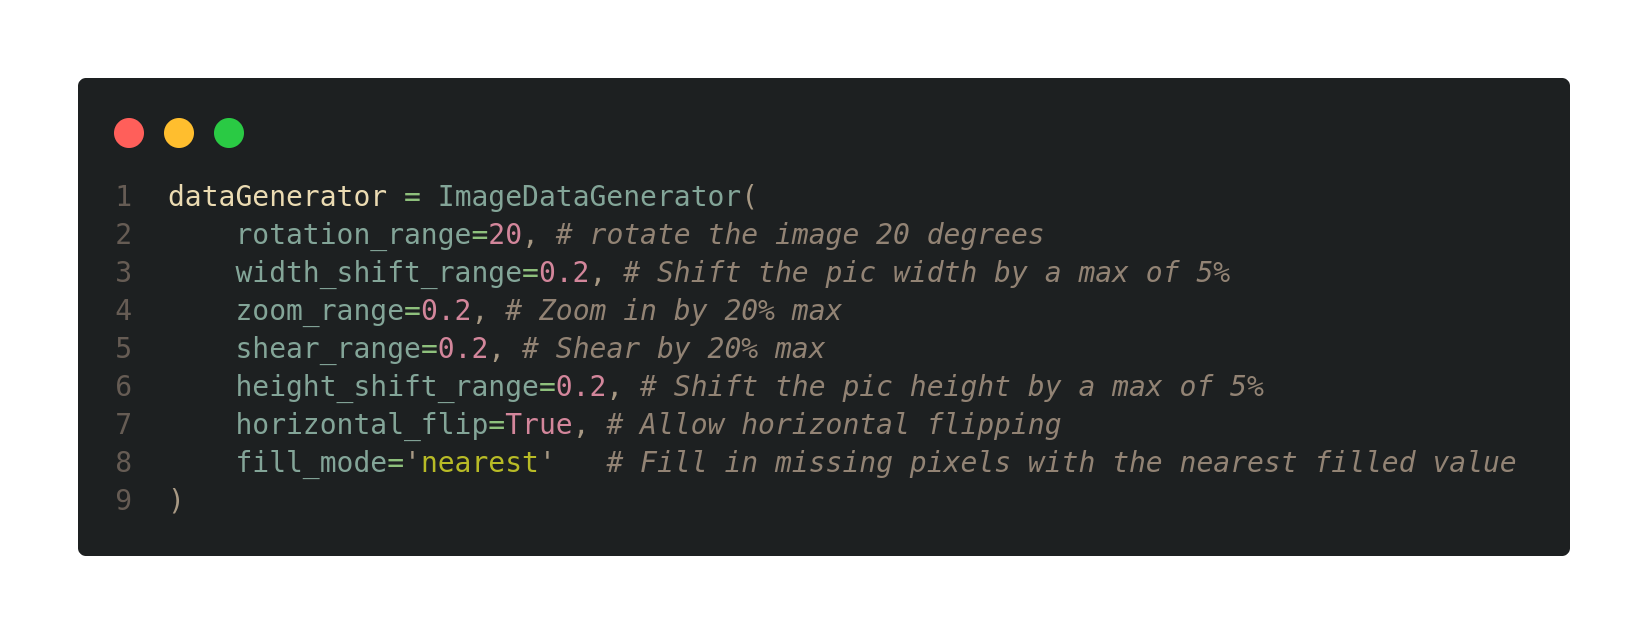
\includegraphics[width=1\linewidth]{images/modelo_aulas_dataaug.png}
    \caption{Data Augmentation Applied}
    \label{fig:enter-label}
\end{figure}

The next figure provides a visual representation of the accuracy and loss trends for both training and validation data across the \textbf{10 epochs}, offering insights into the model's learning dynamics.

\begin{figure}[H]
    \centering
    \begin{subfigure}[t]{0.45\textwidth} % Tamanho de cada subfigura
        \centering
        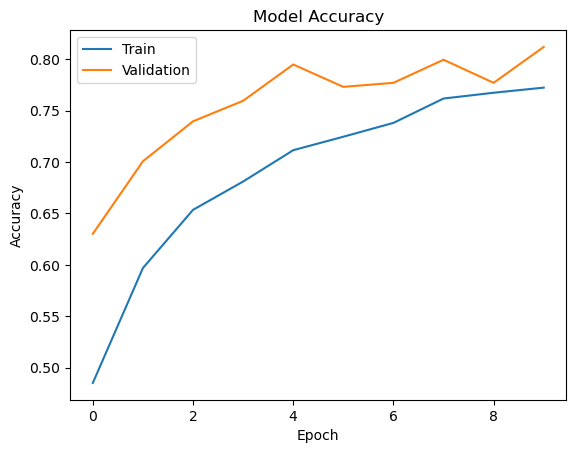
\includegraphics[width=\textwidth]{images/modelo_aula_accuracy_dataaug.png}
        \caption{Train vs Validation Accuracy}
        \label{fig:subfig1}
    \end{subfigure}
    \hfill
    \begin{subfigure}[t]{0.45\textwidth}
        \centering
        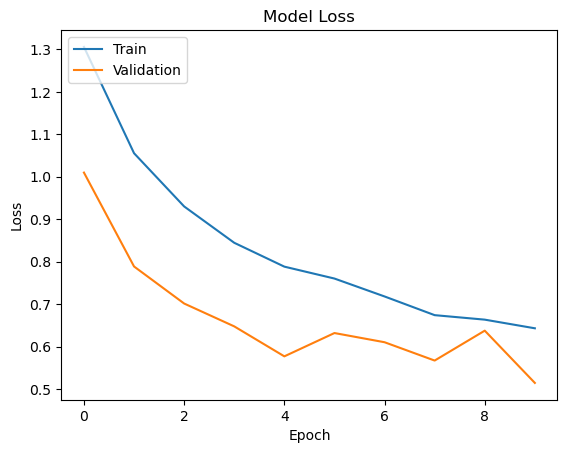
\includegraphics[width=\textwidth]{images/modelo_aula_loss_dataaug.png}
        \caption{Train vs Validation Loss}
        \label{fig:subfig2}
    \end{subfigure}
    \caption{Accuracy and Loss for the First Model with Data Augmentation}
    \label{fig:images}
\end{figure}

The graphs reveal that, unlike the model without data augmentation, the discrepancy between training and validation performance is no longer evident. The training accuracy consistently improves while the validation accuracy closely follows, remaining slightly higher throughout the epochs. Additionally, the training and validation loss curves align more closely, indicating that the model benefits from the data augmentation, reducing overfitting and generalizing better to unseen data.

To gain a deeper understanding of the model's performance, we generated the confusion matrix for the test data and calculated the precision, recall, and F1-score, providing a more comprehensive evaluation of the model's effectiveness across different classes.

\begin{figure}[H]
    \centering
    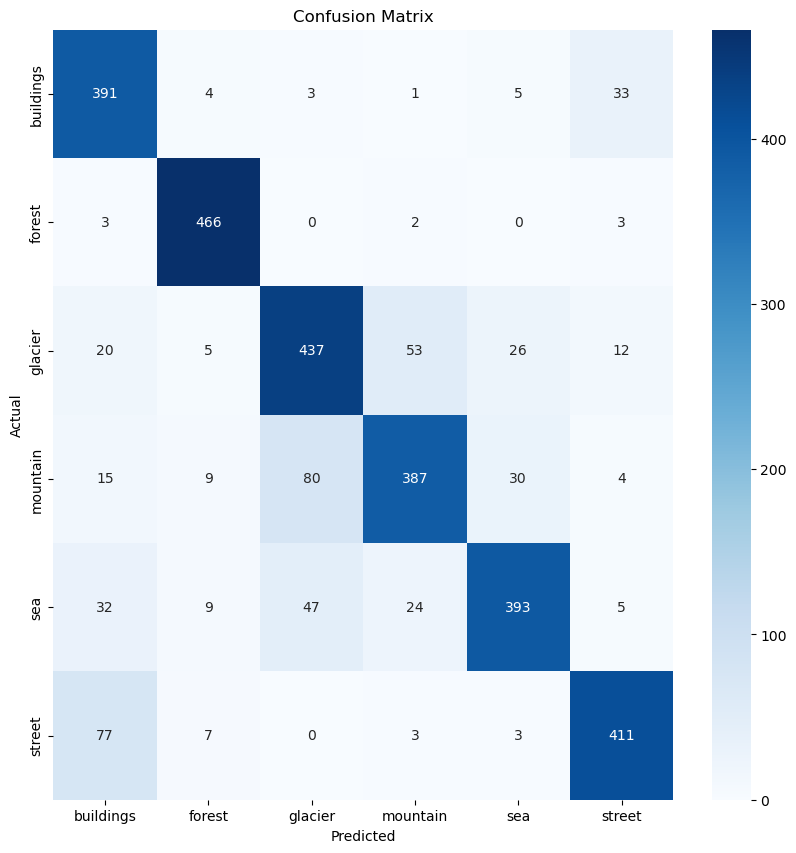
\includegraphics[width=1\linewidth]{images/modelos_aula_confusion_dataaug.png}
    \caption{Model Confusion Matrix}
    \label{fig:enter-label}
\end{figure}

\begin{figure}[H]
    \centering
    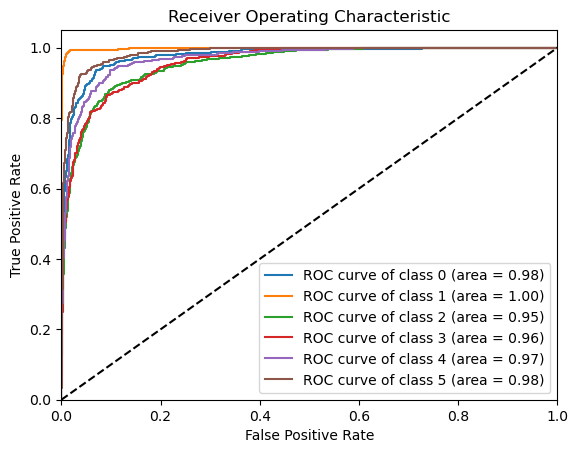
\includegraphics[width=1\linewidth]{images/modelo_aula_roc_dataaug.png}
    \caption{Roc Curve}
    \label{fig:rocincial}
\end{figure}

\begin{table}[H]
    \centering
    \caption{Model Test Evaluation Metrics} 
    \begin{tabular}{||c|c|c|c|c||} 
        \hline
        Accuracy & F1 Score & Recall & Precision \\
        \hline\hline
        0.823 & 0.828 & 0.829 & 0.832 \\
        \hline
    \end{tabular}
    \label{tab:tab_LogReg}
\end{table}


With the inclusion of data augmentation, the model continues to face challenges in distinguishing certain categories. Specifically, Streets (5) are still frequently misclassified as Buildings (0), with 77 instances of such misclassification. Similarly, the confusion between Mountains (3) and Glaciers (2) persists, as well as between Sea (4) and Glaciers (2), reflecting ongoing difficulties in differentiating visually similar categories.

While it was anticipated that data augmentation would lead to improvements in evaluation metrics such as precision, recall, F1-score, and accuracy, the results showed that these metrics remained relatively unchanged. This indicates that although data augmentation helped in diversifying the training data, it did not significantly enhance the model's ability to resolve the inherent challenges of certain class distinctions.

The ROC (Receiver Operating Characteristic) curves for the six scene classes provide a comprehensive overview of the model’s ability to differentiate between various types of scenery. Each curve plots the true positive rate against the false positive rate, with the Area Under the Curve (AUC) indicating the model’s performance.

With data augmentation, the ROC curves improved across most classes, except for class 2 (Glacier), where the AUC value decreased slightly, and in some cases, the values remained unchanged. Notably, class 1 (Forest) continued to demonstrate the best AUC value, showcasing the model's strength in accurately classifying this category. 

\subsection{Feedforward Neural Networks (FNNs)}
Following the CNN Class with Data Augmentation, we explored Feedforward Neural Networks. This FNN approach uses Data Augmentation to techniques which are exhibited in the following image.
\begin{figure}[H]
    \centering
    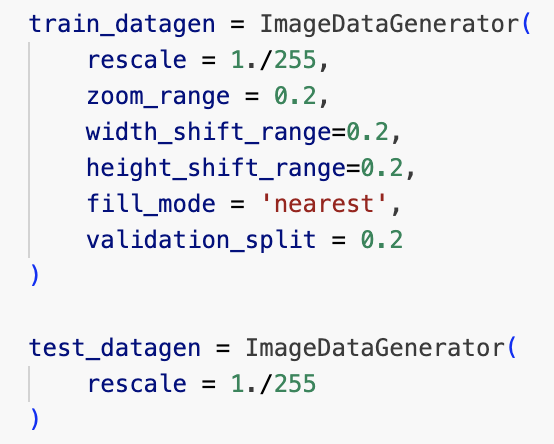
\includegraphics[width=0.5\linewidth]{images/fnn_data_aug.png}
    \caption{Data Augmentation techniques that were used.}
    \label{fig:FNN_data_aug}
\end{figure}
The techniques used include random zooms in or out on the images by up to 20\%, random shifts of the image horizontally and vertically up to 20\%, and a strategy that fills the missing pixels created by zooms and other transformations using the nearest pixel values.

The implemented FNN model includes an input layer, three hidden layers, and an output layer. As with the previous CNN, the model was compiled using the Adam optimizer and the loss function is the "categorical crossentropy".

A grid search approach of hypertuning the model was used. It consisted of trying out different values of the hyperparameters and picking the "model" that gives the best score. This approach was used for balancing computational efficiency and thoroughness in exploring hyperparameter combinations. The hyperparameters that were tuned are the number of neurons per hidden layer and the activation function of the hidden layers. The values experimented of each hyperparameter can be consulted in the table \ref{tab:fnn_hypertuning}.

\begin{table}[H]
\centering
\caption{FNN tuned hyperparameters.}
\begin{tabular}{|l|c|}
\hline
\textbf{Hyperparameter} & \textbf{Values} \\ \hline
Number of neurons per hidden layer & \{25, 50, 100, 200\} \\ \hline
Activation & \{ReLU, Sigmoid\} \\ \hline
\end{tabular}
\label{tab:fnn_hypertuning}
\end{table}

For each model created with a different set of hyperparameters the test confusion matrix and performance metrics were registered. This registration was made with the help of TensorBoard. Tensorboard is a python package that provides "visualization and tooling needed for machine learning experimentation"\cite{tensorboard}. It was instrumental in monitoring training and validation loss curves, ensuring proper convergence. The results for each model are kept in a logs folder which facilitates its detailed analysis.

In the image \ref{fig:FNN_table} all the performance metrics evaluated along with the tuned hyperparameters are exhibited.
\begin{figure}[H]
    \centering
    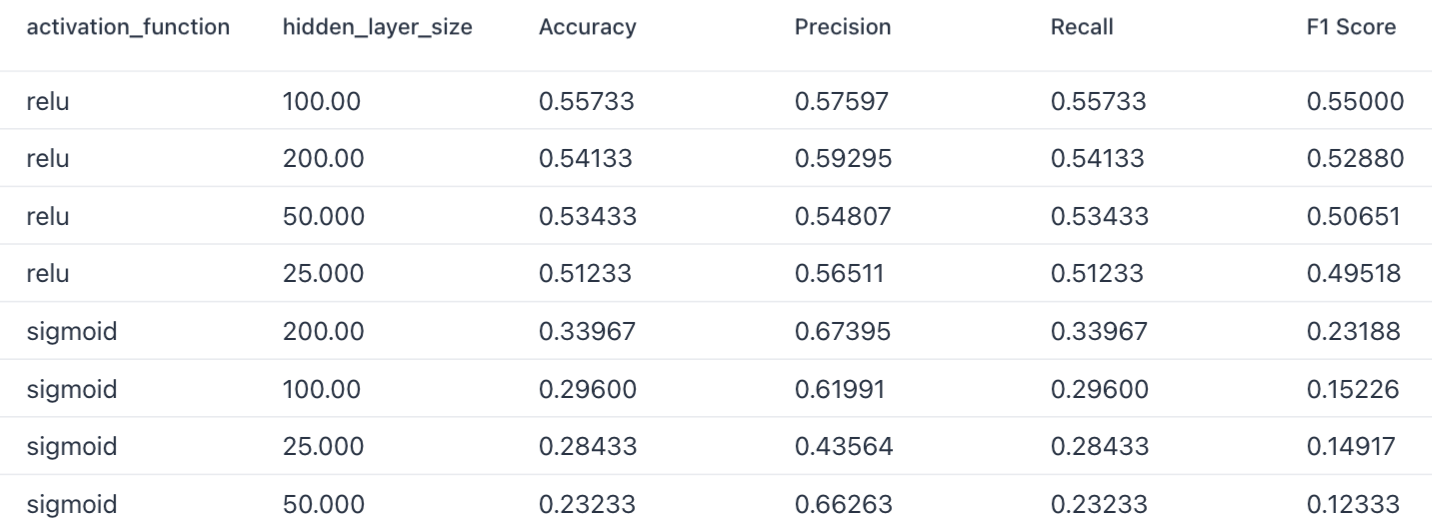
\includegraphics[width=1\linewidth]{images/FNN_tensorboard_table.png}
    \caption{Table containing the hyperparameters and the results of the hypertuning process performed.}
    \label{fig:FNN_table}
\end{figure}
The first model present in the image stands out as the best combination of tuned hyperparameters as it has the best results regarding the performance metrics. This model uses 100 neurons for each hidden layer, and a relu activation function in the three hidden layers. 

The best performance for relu is achieved with a hidden layer size of 100, with the following metrics:
\begin{itemize}
    \item Accuracy: 0.55733
    \item Precision: 0.57597
    \item Recall: 0.55733
    \item F1 Score: 0.55000
\end{itemize}

Sigmoid’s best performance is with a hidden layer size of 200, but its metrics are significantly lower:
\begin{itemize}
    \item Accuracy: 0.33967
    \item Precision: 0.67395
    \item Recall: 0.33967
    \item F1 Score: 0.23188
\end{itemize}

The relu activation function consistently outperforms sigmoid, even the best sigmoid model performs worse than any relu model. This is likely due to its ability to prevent vanishing gradient issues compared to sigmoid. When calculating the gradient for sigmoid its derivative is at most 0.25. The down side of this is when you have many layers the multiplication of these gradients tend to zero very quickly \cite{vanishing_grad}. 

The next figure provides a visual representation of the accuracy and loss trends for both training and validation data across the hyperparameter model over \textbf{30 epochs}, offering insights into the model's learning dynamics.

\begin{figure}[H]
    \centering
    \begin{subfigure}[t]{0.35\textwidth} % Tamanho de cada subfigura
        \centering
        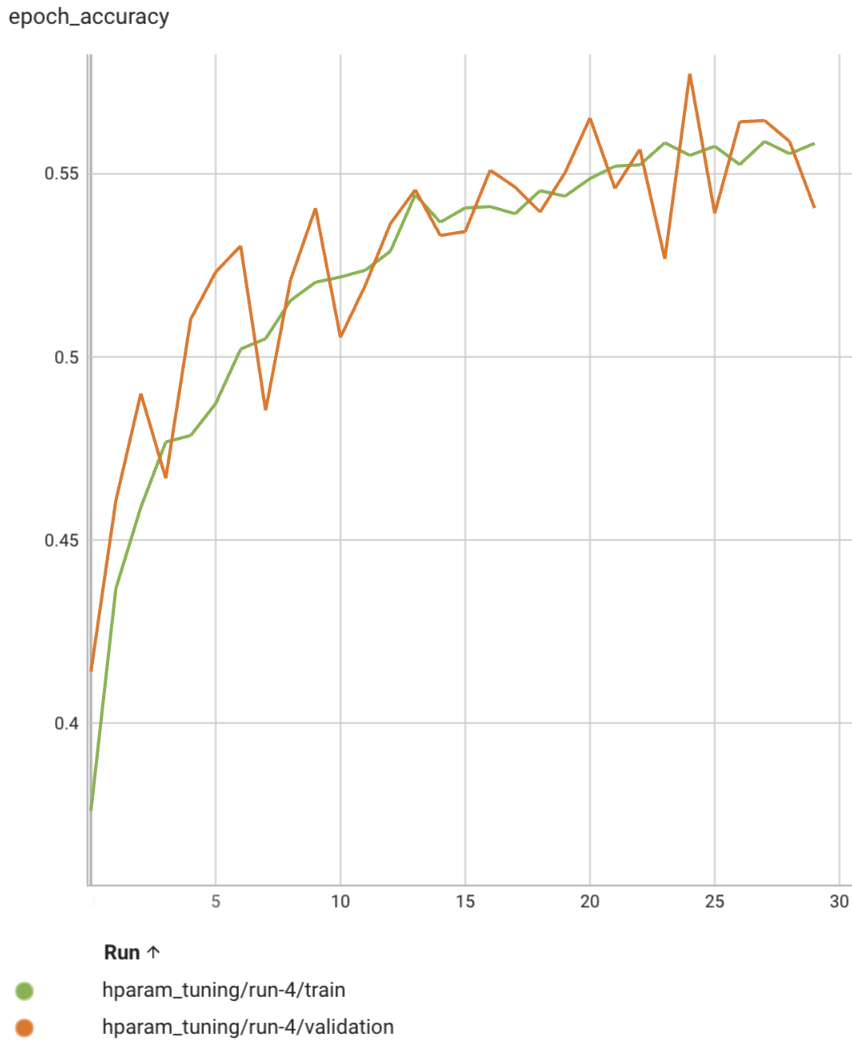
\includegraphics[width=\textwidth]{images/fnn_epoch_accuracy.png}
        \caption{Train vs Validation Accuracy over epochs}
        \label{fig:fnn_subfig1}
    \end{subfigure}
    \hfill
    \begin{subfigure}[t]{0.30\textwidth}
        \centering
        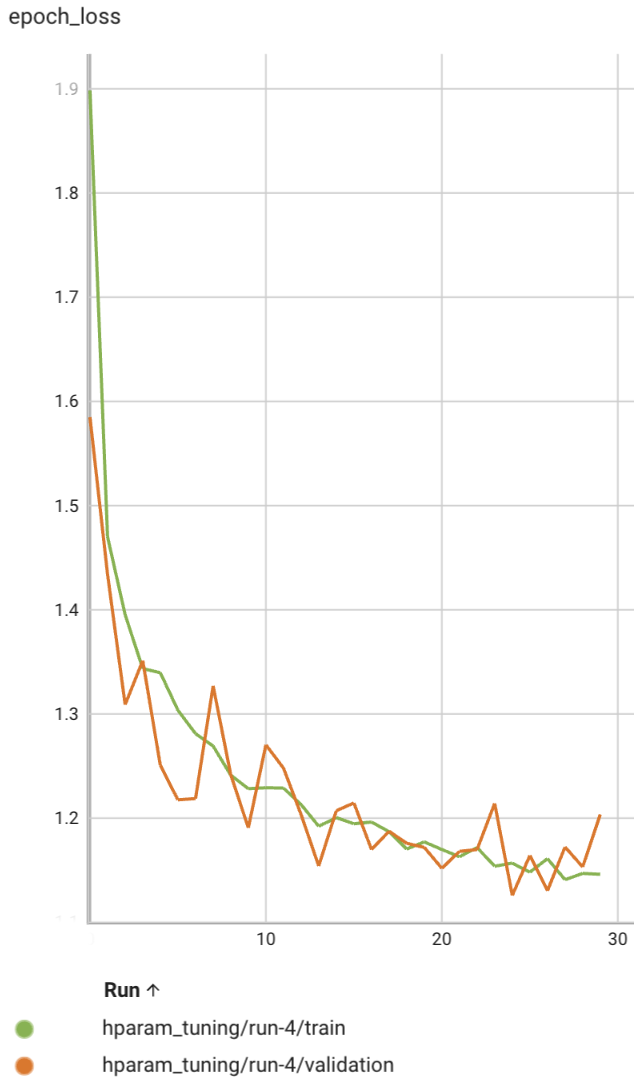
\includegraphics[width=\textwidth]{images/fnn_epoch_loss.png}
        \caption{Train vs Validation Loss over epochs}
        \label{fig:fnn_subfig2}
    \end{subfigure}
    \caption{Accuracy and Loss over epoch for the best set of hyperparameters FNN model.}
    \label{fig:images}
\end{figure}

As we can see in the first chart the training stabilizes by the 20th epoch, indicating that further training brings no significant improvements. The validation accuracy follows a similar trend to the training accuracy, increasing steadily during the early epochs. However, it also stabilizes after the 20th epoch. Both training and validation accuracies converge near the end of training. This suggests the model's performance on the validation set is close to that on the training set, suggesting good generalization. We can see there is little to no gap in both images between the training and validation curves which indicates the model does not overfit the training data.

To gain a deeper understanding of the model's performance, we can analyze the generated confusion matrix for the test data in the following image.
\begin{figure}[H]
    \centering
    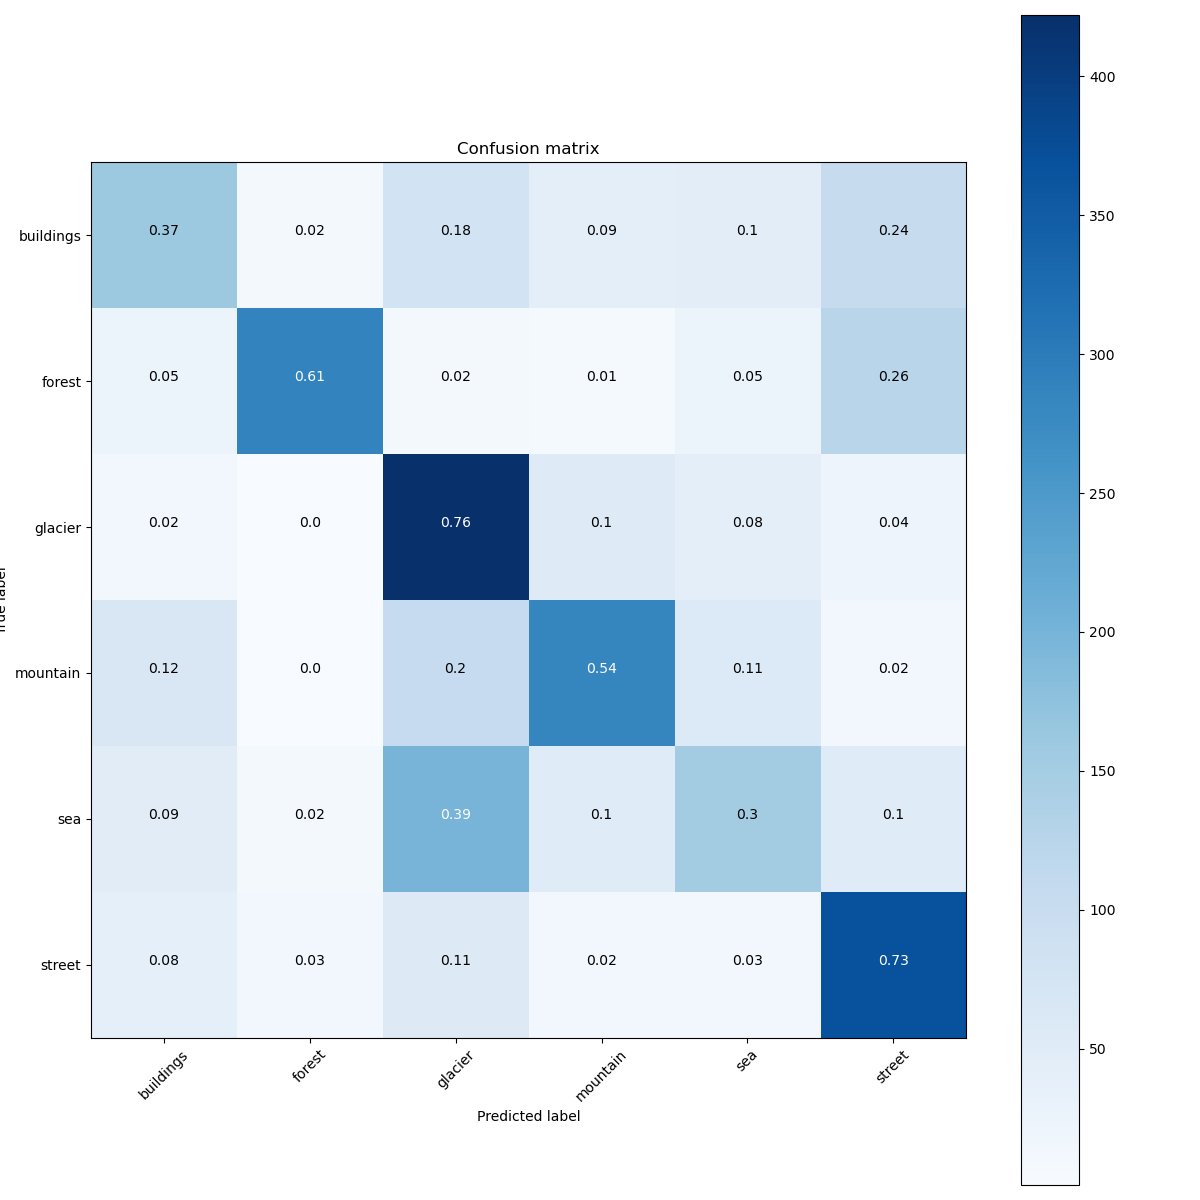
\includegraphics[width=1\linewidth]{images/fnn_cm.png}
    \caption{Confusion matrix of the best hyperparameter FNN model.}
    \label{fig:FNN_cm}
\end{figure}
This confusion matrix indicates the classes with the highest correct prediction rates are glacier and street, and the more challenging classes are buildings and sea. 

\subsection{Convolutional Neural Networks (CNNs)}
This CNNs approach uses a Data Augmentation training and validation set which is similar to the one used in the FNN approach described before.

The model architecture includes three convolutional layers, each followed by a max-pooling layer, with a fully connected dense layer and a dropout layer for regularization before the output layer. It is structured in the following table.

\begin{table}[H]
\centering
\caption{Architecture of the CNN Model}
\begin{tabular}{|l|}
\hline
\textbf{Layer (Type)}\\ \hline
Conv2D                      \\ \hline
MaxPooling2D                \\ \hline
Conv2D                      \\ \hline
MaxPooling2D                \\ \hline
Conv2D                      \\ \hline
MaxPooling2D                \\ \hline
Flatten                     \\ \hline
Dense                       \\ \hline
Dropout                     \\ \hline
Dense                  \\
\hline
\end{tabular}
\label{tab:cnn_architecture_2}
\end{table}

A grid search approach of hypertuning the model was used. It consisted of trying out different values of the hyperparameters and picking the "model" that gives the best score. This approach was used for balancing computational efficiency and thoroughness in exploring hyperparameter combinations. The hyperparameters that were tuned are the kernel/filter size, the dropout rate, and the optimizer function. The values experimented of each hyperparameter can be consulted in the table \ref{tab:cnn_hypertuning}.

\begin{table}[H]
\centering
\caption{CNN tuned hyperparameters.}
\begin{tabular}{|l|c|}
\hline
\textbf{Hyperparameter} & \textbf{Values} \\ \hline
Filter size & \{3, 5, 7\} \\ \hline
Dropout rate & \{0.2, 0.5\} \\ \hline
Otimizer & \{adam, sgd\} \\ \hline
\end{tabular}
\label{tab:cnn_hypertuning}
\end{table}

For each model created with a different set of hyperparameters the test confusion matrix and performance metrics were registered. This registration was made with the help of TensorBoard. Tensorboard is a python package that provides "visualization and tooling needed for machine learning experimentation"\cite{tensorboard}. It was instrumental in monitoring training and validation loss curves, ensuring proper convergence. The results for each model are kept in a logs folder which facilitates its detailed analysis.

In the image \ref{fig:CNN_table} all the performance metrics evaluated along with the tuned hyperparameters are exhibited.
\begin{figure}[H]
    \centering
    \includegraphics[width=1\linewidth]{images/CNN_tensorboard_table.png}
    \caption{Table containing the hyperparameters and the results of the hypertuning performed.}
    \label{fig:CNN_table}
\end{figure}
The first model present in the image stands out as the best combination of tuned hyperparameters as it has the best results regarding the performance metrics. It uses the adam optimizer, a kernel size of 3, and a dropout rate of 0.5. From the results we can understand that Adam consistently outperforms SGD. Smaller kernel sizes (3 or 5) generally perform better, with Adam paired with kernel size of 3 being the most effective.

The next figure provides a visual representation of the accuracy and loss trends for both training and validation data across the hyperparameter model over \textbf{30 epochs}, offering insights into the model's learning dynamics.

\begin{figure}[H]
    \centering
    \begin{subfigure}[t]{0.35\textwidth} % Tamanho de cada subfigura
        \centering
        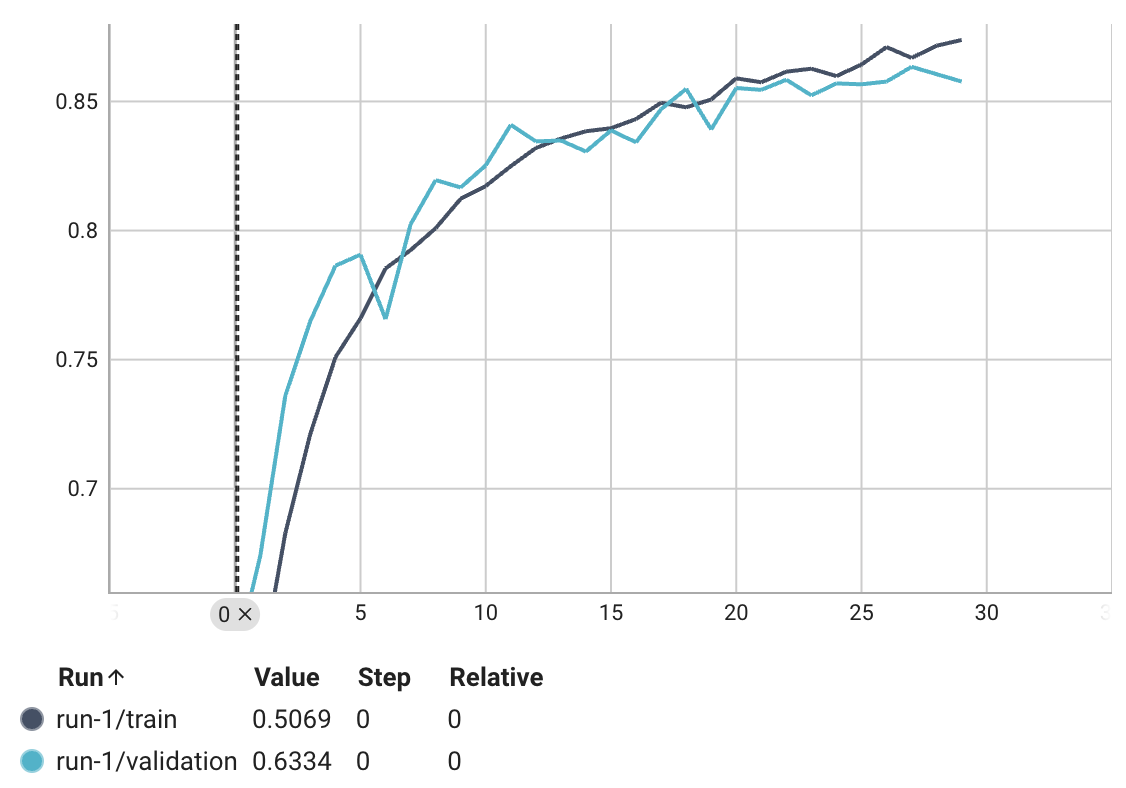
\includegraphics[width=\textwidth]{images/cnn_epoch_accuracy.png}
        \caption{Train vs Validation Accuracy over epochs}
        \label{fig:cnn_subfig1}
    \end{subfigure}
    \hfill
    \begin{subfigure}[t]{0.30\textwidth}
        \centering
        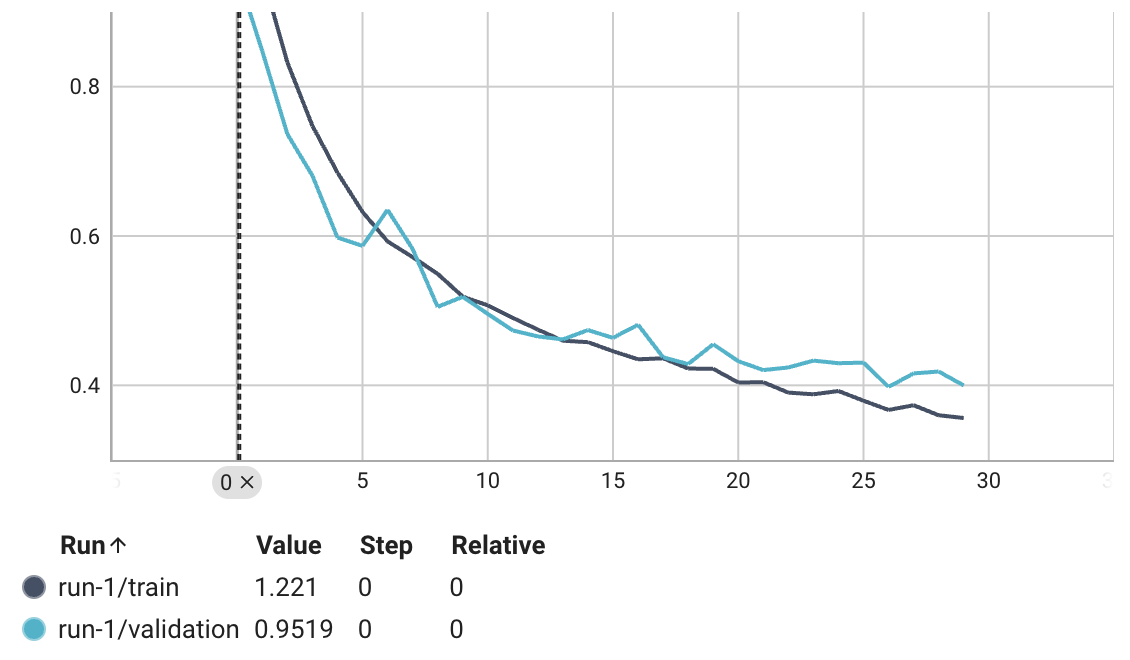
\includegraphics[width=\textwidth]{images/cnn_epoch_loss.png}
        \caption{Train vs Validation Loss over epochs}
        \label{fig:cnn_subfig2}
    \end{subfigure}
    \caption{Accuracy and Loss over epoch for the best set of hyperparameters CNN model.}
    \label{fig:images}
\end{figure}

As we can see in the first chart the training stabilizes by the 20th epoch, indicating that further training brings no significant improvements. The validation accuracy follows a similar trend to the training accuracy, increasing steadily during the early epochs. However, it also stabilizes after the 20th epoch. Both training and validation accuracies converge near the end of training. This suggests the model's performance on the validation set is close to that on the training set, suggesting good generalization. We can see there is little to no gap in both images between the training and validation curves which indicates the model does not overfit the training data.

To gain a deeper understanding of the model's performance, we can analyze the generated confusion matrix for the test data in the following image.
\begin{figure}[H]
    \centering
    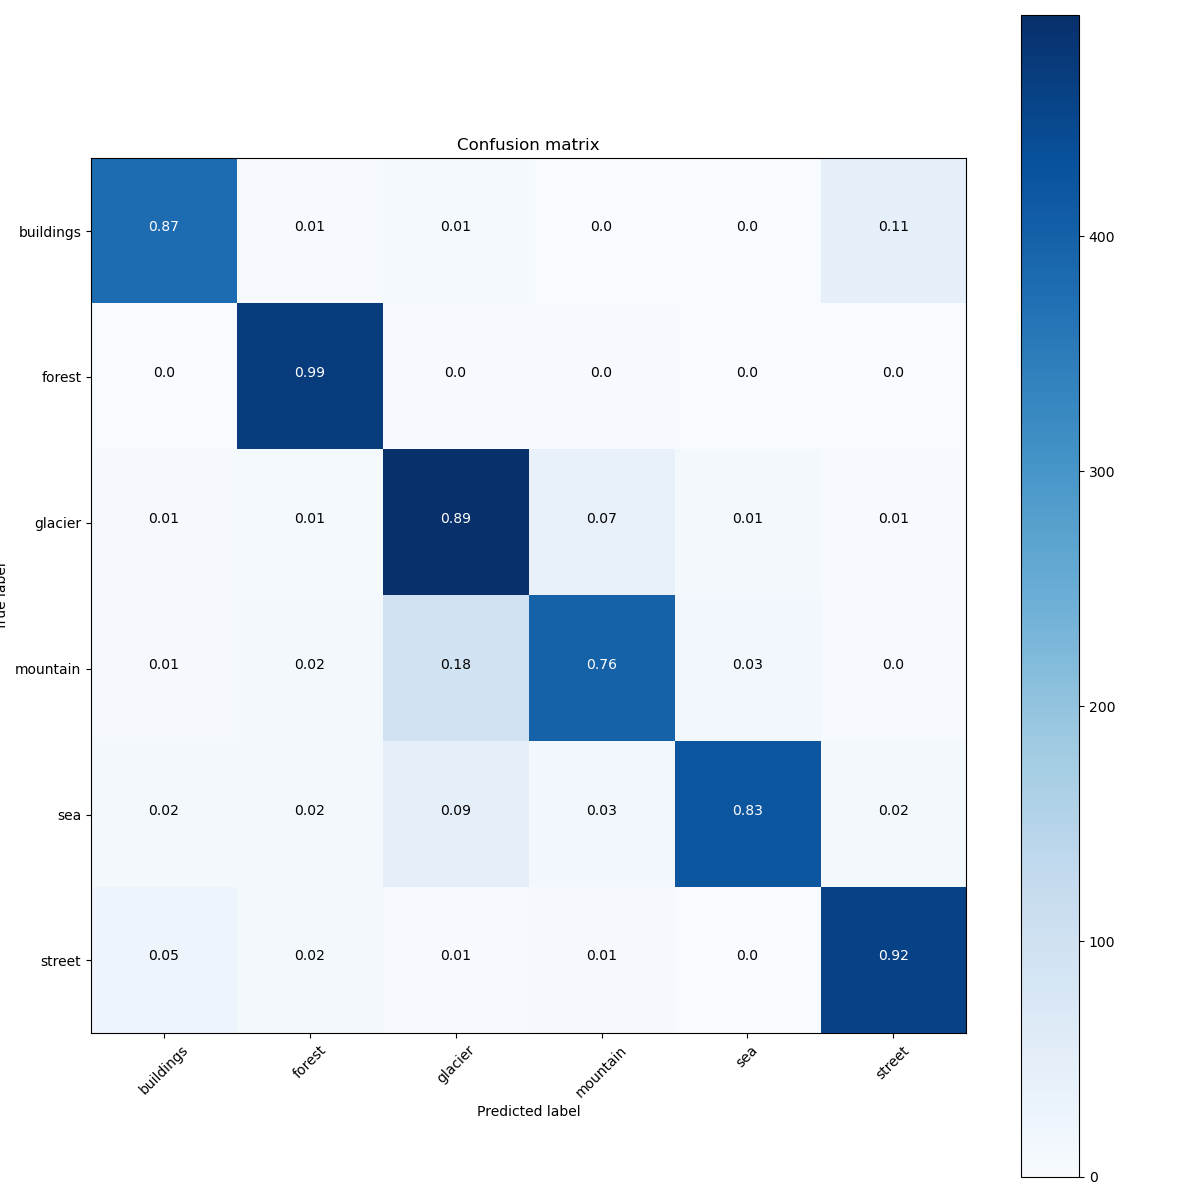
\includegraphics[width=1\linewidth]{images/cnn_tensorboard_cm.png}
    \caption{Confusion matrix of the best hyperparameter CNN model.}
    \label{fig:CNN_cm}
\end{figure}

The confusion matrix indicates the model performs exceptionally well on Forest and Street classes, suggesting strong feature extraction and learning for these categories. Overall there is minimal missclassifications which highlights the robustness of the model in distinguishing between classes.
The largest source of misclassification are mountains vs glaciers, 18\% of mountains are predicted as glaciers. This suggests overlapping features or insufficiently distinct feature extraction for these classes. The 11\% missclassification rate for buildings as streets show that urban environments are challenging to classify.

\subsection{DenseNet Model}

This model utilizes the DenseNet121 architecture, which is a deep convolutional network designed to improve feature reuse through dense connections. Instead of using simple convolutional layers, DenseNet121 employs a more complex design with dense blocks, where each layer receives input from all previous layers, allowing the model to learn more complex representations while reducing the number of parameters.

In this implementation, the pre-trained weights from ImageNet are used for feature extraction. The DenseNet121 model is fine-tuned by adding a Global Average Pooling layer followed by a fully connected dense layer with 128 units and a ReLU activation. To prevent overfitting, a Dropout layer with a rate of 0.5 is applied before the final output layer. The output layer consists of 6 units with a Softmax activation, designed to classify the images into one of six categories.

The model was compiled using the Adam optimizer with a default learning rate of 0.001. The Adam optimizer is well suited for this task due to its adaptive learning rate capabilities.
The loss function used is ”categorical crossentropy”, which is appropriate for multiclass classification problems, and the performance metric tracked during training was accuracy.
The performance of the DenseNet model was evaluated using training, validation, and test datasets. The model demonstrated a high accuracy on the training data but showed a significant drop in accuracy on the validation and test data, indicating potential overfitting.

The next figure provides a visual representation of the accuracy and loss trends for both training and validation data across the \textbf{30 epochs}, offering insights into the model's learning dynamics.
The model achieved higher accuracy on the training data compared to the validation and test data. This discrepancy suggests potential overfitting, where the model performs well on the data it has seen but struggles to generalize effectively to unseen data.
This behavior is further corroborated by the loss values recorded during training and validation, which highlight the challenges in maintaining consistency across datasets.

\begin{figure}[H]
    \centering
    \begin{subfigure}[t]{0.45\textwidth} 
        \centering
        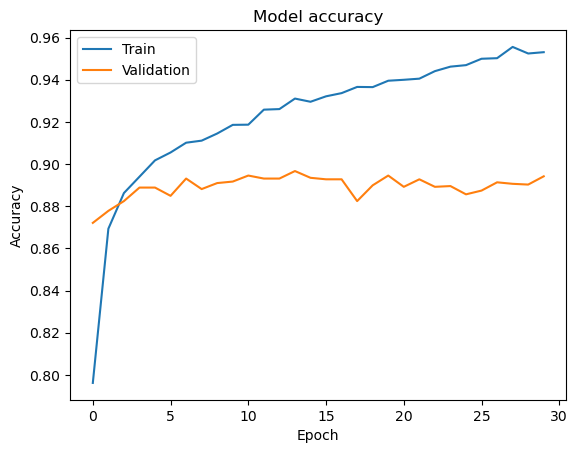
\includegraphics[width=\textwidth]{images/densenet_accuracy.png}
        \caption{Train vs Validation Accuracy}
        \label{fig:subfig1}
    \end{subfigure}
    \hfill
    \begin{subfigure}[t]{0.45\textwidth}
        \centering
        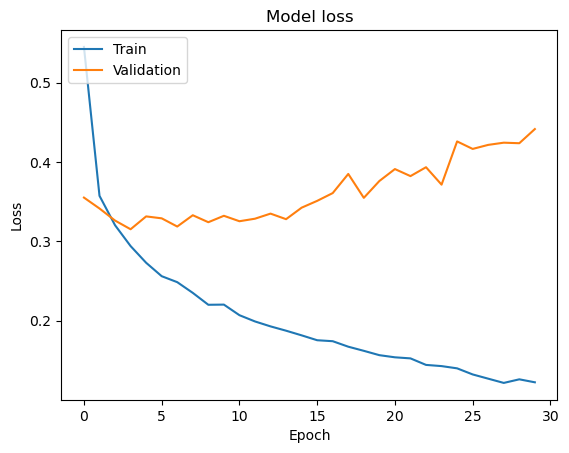
\includegraphics[width=\textwidth]{images/densenet_loss.png}
        \caption{Train vs Validation Loss}
        \label{fig:subfig2}
    \end{subfigure}
    \caption{Accuracy and Loss for the DenseNet Model}
    \label{fig:images}
\end{figure}

The graphs reveal that while the training accuracy consistently improves and the training loss decreases, the validation accuracy stagnates after the initial epochs, and the validation loss increases. This pattern further reinforces the indication of overfitting.

To gain a deeper understanding of the model's performance, we generated the confusion matrix for the test data and calculated the precision, recall, and F1-score, providing a more comprehensive evaluation of the model's effectiveness across different classes.


\begin{figure}[H]
    \centering
    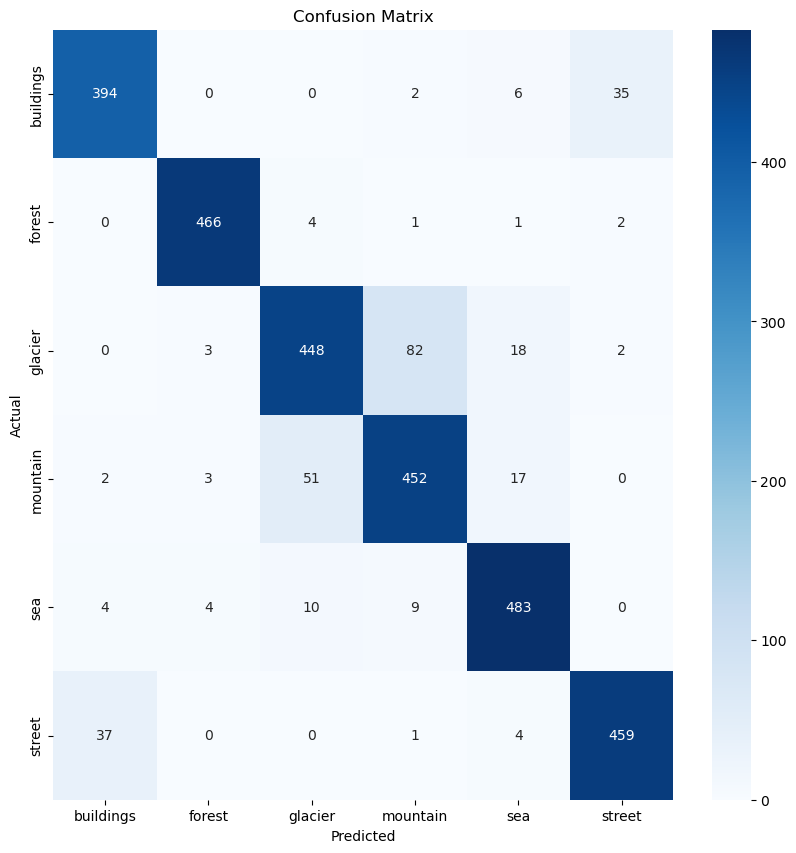
\includegraphics[width=1\linewidth]{images/densenet_confusion.png}
    \caption{Model Confusion Matrix}
    \label{fig:enter-label}
\end{figure}

\begin{figure}[H]
    \centering
    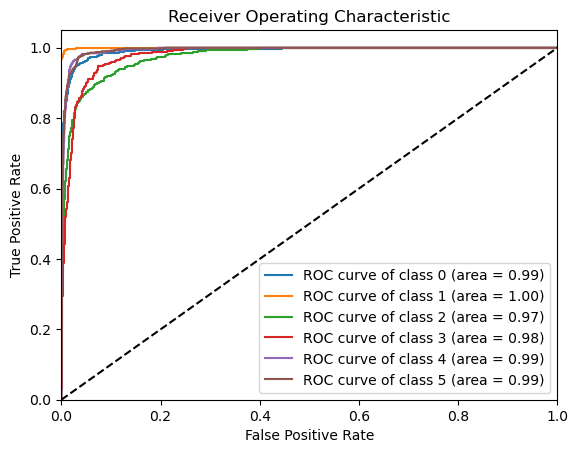
\includegraphics[width=1\linewidth]{images/densenet_roc.png}
    \caption{Roc Curve}
    \label{fig:rocincial}
\end{figure}

\begin{table}[H]
    \centering
    \caption{Model Test Evaluation Metrics} 
    \begin{tabular}{||c|c|c|c|c||} 
        \hline
        Accuracy & F1 Score & Recall & Precision \\
        \hline\hline
        0.900 & 0.900 & 0.901 & 0.901 \\
        \hline
    \end{tabular}
    \label{tab:tab_LogReg}
\end{table}

Forests (1) are classified very accurately, with the majority of predictions falling into the correct category. Buildings (0), however, are still often misclassified as Streets (5), with 35 misclassifications, and Streets (5) are sometimes confused with Buildings (0). Despite these challenges, the model shows significant improvements in overall performance. However, there remains a notable overlap between certain classes. Mountains (3) and Glaciers (2) are still frequently confused with each other, reflecting their visual similarities, with 82 mountains misclassified as glaciers and 51 glaciers misclassified as mountains. Similarly, there is still confusion between Streets (5) and Buildings (0), highlighting the difficulty in distinguishing these two categories due to their structural similarities in the dataset.

The ROC (Receiver Operating Characteristic) curves for the six scene classes provide an overall view of the model’s ability to distinguish between different types of scenery. Each ROC curve plots the true positive rate against the false positive rate, with the Area Under the Curve (AUC) representing the
model’s performance. As it can be seen in the ROC curve, all classes, except for Glaciers (2), performed very closely to achieving perfect results, with only minor deviations. Class 1 (Forest) achieved the best AUC value, showing the highest accuracy in distinguishing its category. However, Glaciers (2) fell short in comparison to the other categories, with a significantly lower AUC score, indicating more difficulty in distinguishing this class from the others.


\subsection{DenseNet with Data Augmentation}

This model follows the same architecture as the previous model, but with the addition of data augmentation to enhance the model's ability to generalize. Data augmentation techniques, including random rotations, width and height shifts, zooming, shearing, and horizontal flipping, were applied to the training data. These transformations aim to create a more diverse set of images for training, which helps in reducing overfitting.


\begin{figure}[H]
    \centering
    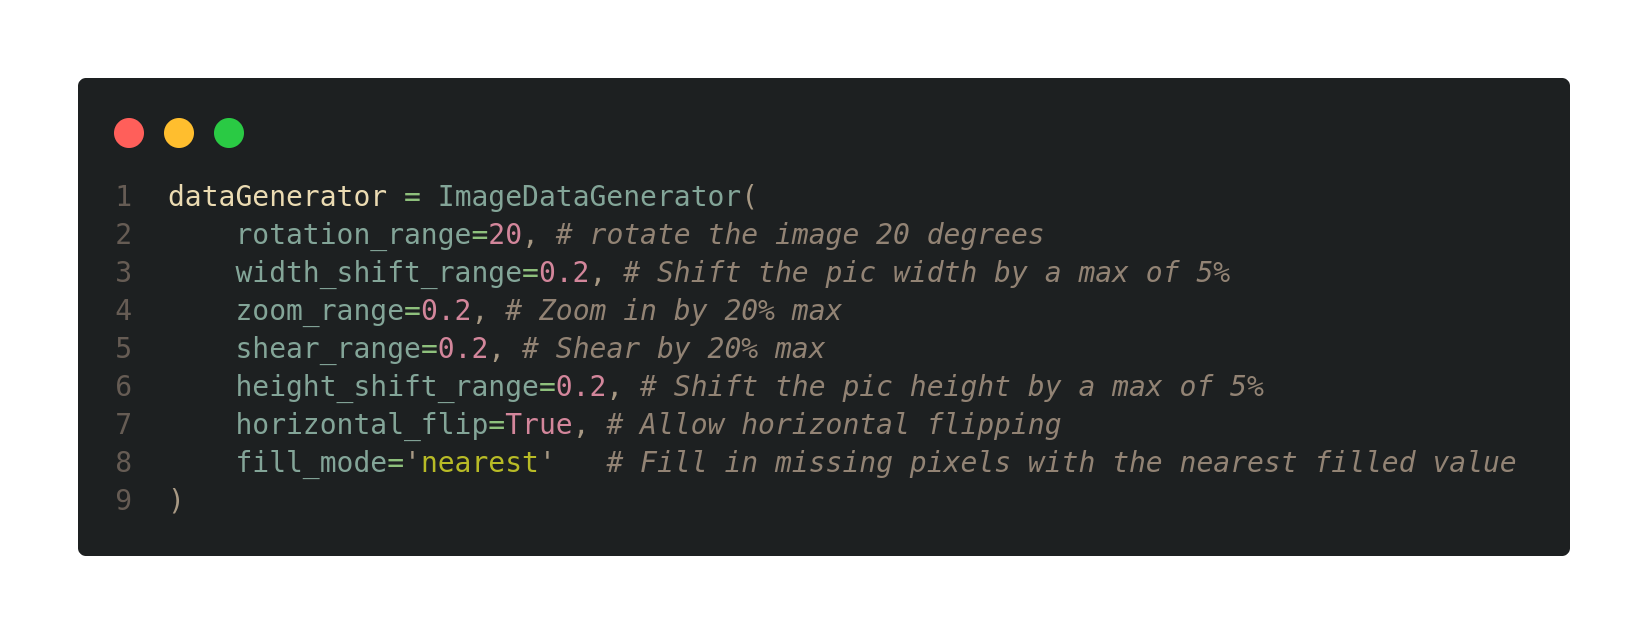
\includegraphics[width=1\linewidth]{images/modelo_aulas_dataaug.png}
    \caption{Data Augmentation Applied}
    \label{fig:enter-label}
\end{figure}

The next figure provides a visual representation of the accuracy and loss trends for both training and validation data across the \textbf{30 epochs}, offering insights into the model's learning dynamics.


\begin{figure}[H]
    \centering
    \begin{subfigure}[t]{0.45\textwidth} 
        \centering
        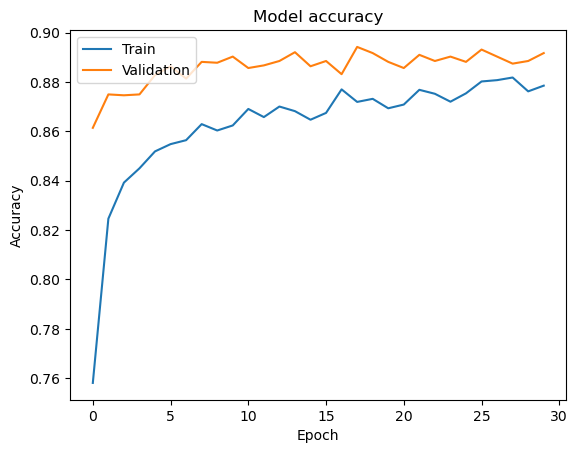
\includegraphics[width=\textwidth]{images/densenet_accuracy_dataaug.png}
        \caption{Train vs Validation Accuracy}
        \label{fig:subfig1}
    \end{subfigure}
    \hfill
    \begin{subfigure}[t]{0.45\textwidth}
        \centering
        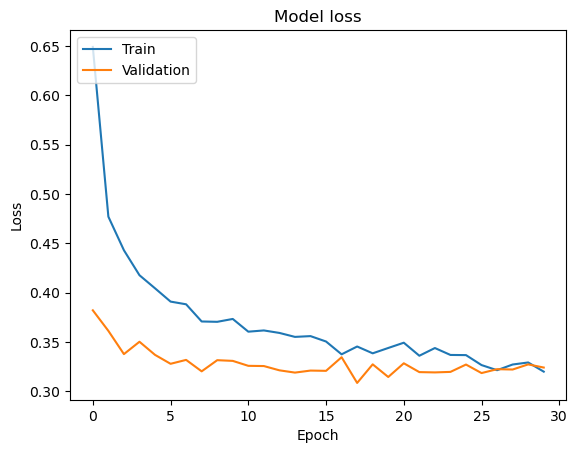
\includegraphics[width=\textwidth]{images/densenet_loss_dataaug.png}
        \caption{Train vs Validation Loss}
        \label{fig:subfig2}
    \end{subfigure}
    \caption{Accuracy and Loss for the DenseNet Model with Data Augmentation}
    \label{fig:images}
\end{figure}

The graphs reveal that, unlike the model without data augmentation, the discrepancy between training and validation performance is no longer evident. The training accuracy consistently improves while the validation accuracy closely follows, remaining slightly higher throughout the epochs. Additionally, the training and validation loss curves align more closely, indicating that the model benefits from the data augmentation, reducing overfitting and generalizing better to unseen data.

To gain a deeper understanding of the model's performance, we generated the confusion matrix for the test data and calculated the precision, recall, and F1-score, providing a more comprehensive evaluation of the model's effectiveness across different classes.


\begin{figure}[H]
    \centering
    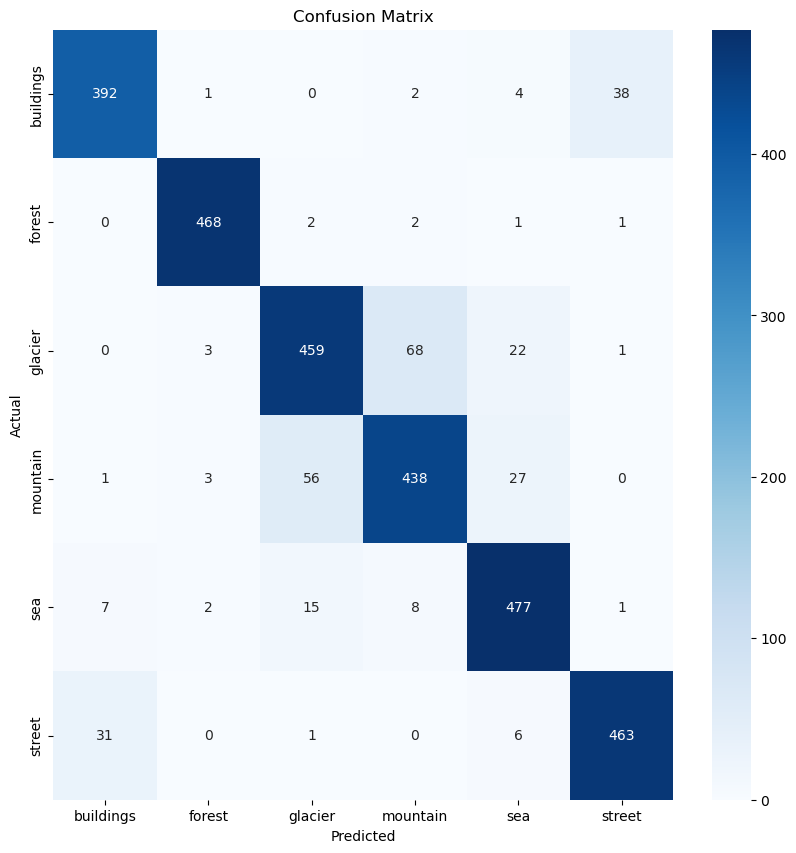
\includegraphics[width=1\linewidth]{images/densenet_confusion_dataug.png}
    \caption{Model Confusion Matrix}
    \label{fig:enter-label}
\end{figure}
\begin{figure}[H]
    \centering
    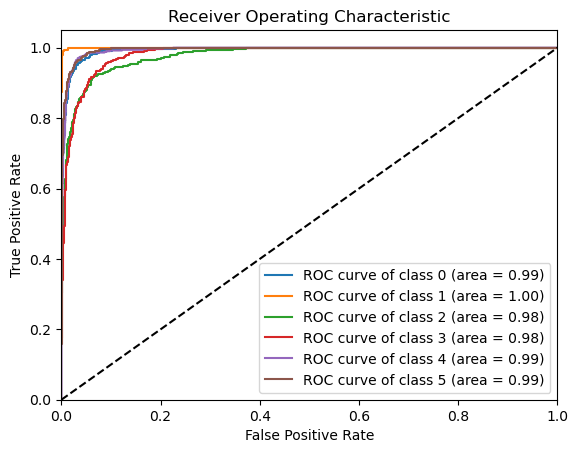
\includegraphics[width=1\linewidth]{images/densenet_roc_aug.png}
    \caption{Roc Curve}
    \label{fig:rocincial}
\end{figure}

\begin{table}[H]
    \centering
    \caption{Model Test Evaluation Metrics} 
    \begin{tabular}{||c|c|c|c|c||} 
        \hline
        Accuracy & F1 Score & Recall & Precision \\
        \hline\hline
        0.899 & 0.899 & 0.899 & 0.899 \\        
        \hline
    \end{tabular}
    \label{tab:tab_LogReg}
\end{table}



With the DenseNet model and data augmentation applied, Forests (1) remain the best-classified category, with the majority of predictions falling correctly into this class. Additionally, Sea (4) also demonstrates strong performance, showing considerable improvement.

However, the model still struggles to differentiate Buildings (0) and Streets (5), with misclassifications increasing slightly from 35 to 38. The confusion between Glaciers (2) and Mountains (3) persists, though it has improved significantly compared to earlier results. These improvements highlight the potential of DenseNet with data augmentation in addressing some classification challenges while leaving room for further refinement in distinguishing between visually similar categories.

The ROC (Receiver Operating Characteristic) curves for the six scene classes provide an insightful overview of the model’s capacity to differentiate between various types of scenery. Each curve represents the true positive rate against the false positive rate, with the Area Under the Curve (AUC) reflecting overall performance.

With the DenseNet model and data augmentation applied, results remain largely consistent, with notable improvements across some classes. For instance, Glaciers (2), previously a weaker category, now exhibits a much stronger AUC score, with values ranging between 0.98 and 1, demonstrating a significant enhancement in distinguishing this class. Other classes, including Forests (1), continue to show near-perfect performance, maintaining AUC values very close to 1. These results underline the model’s progress in achieving robust classification across most categories.



























\subsection{Comparison between the models}

The comparison between the models is based on the following performance metrics: Accuracy, F1 Score, Recall, and Precision. These metrics allow us to assess how well the models perform in terms of both correctly classifying positive and negative cases and minimizing false positives and false negatives.

\begin{itemize}
    \item \textbf{Accuracy} measures the overall correctness of the model by calculating the ratio of correct predictions to the total number of predictions.
    \item \textbf{F1 Score} is the harmonic mean of Precision and Recall, providing a balance between the two, especially when dealing with imbalanced classes.
    \item \textbf{Recall} (or True Positive Rate) measures the ability of the model to correctly identify positive instances.
    \item \textbf{Precision} measures the accuracy of positive predictions made by the model.
\end{itemize}

\begin{table}[ht]
    \centering
    \caption{Comparison of Models} 
    \begin{tabular}{||c|c|c|c|c||} 
     \hline    
     \textbf{Model} & \textbf{Accuracy} & \textbf{F1 Score} & \textbf{Recall} & \textbf{Precision} \\
     \hline \hline
     CM & 0.834 & 0.834 & 0.834 & 0.835 \\
     \hline
     CM - DA & 0.823 & 0.828 & 0.829 & 0.832 \\
     \hline
          FNN - ReLU & 0.557 & 0.550 & 0.557 & 0.578 \\
     \hline
    CNN - Hyper & 0.875 & 0.875 & 0.875 & 0.879 \\
    \hline
     DN & 0.900 & 0.900 & 0.901 & 0.901 \\
     \hline 
     DN - DA & 0.899 & 0.899 & 0.899 & 0.899 \\
     \hline
\hline
     \multicolumn{5}{||c||}{\textbf{Models Name}} \\
     \hline
     CM & \multicolumn{4}{|l||}{CNN Class Model} \\ 
     \hline
     CM - DA & \multicolumn{4}{|l||}{CNN Class Model with Data Augmentation} \\ 
     \hline
          FNN - ReLU & \multicolumn{4}{|l||}{FNN ReLU Activation Function (Hidden Layer Size 100)} \\ 
     \hline
         CNN - Hyper & \multicolumn{4}{|l||}{Best Hyper Tunned CNN} \\ 
    \hline
     DN & \multicolumn{4}{|l||}{DenseNet Model} \\ 
     \hline
     DN - DA & \multicolumn{4}{|l||}{DenseNet Model with Data Augmentation} \\ 
     \hline

    \end{tabular}
    \label{tab:tab_Final_results}
\end{table}


Based on the results in Table \ref{tab:tab_Final_results}, we can observe the following:

The DenseNet model (DN) achieved the highest accuracy (90.0) among all models tested, indicating its superior ability to capture and utilize complex features within the Intel Image Classification dataset. The model's performance remained robust even with the application of data augmentation (DN - DA), showing a marginal reduction in accuracy to 89.9. This highlights DenseNet's resilience and strong generalization capabilities.

The CNN Class Model (CM) exhibited a respectable accuracy of 83.4, demonstrating the effectiveness of convolutional layers for feature extraction in image classification tasks. However, when data augmentation was applied (CM - DA), the model's accuracy slightly decreased to 82.3. This indicates that while data augmentation can enhance variability in the training set, it may not always lead to improved performance, particularly in simpler CNN architectures.

The hyperparameter-tuned CNN (CNN - Hyper) performed significantly better than the base CNN model, achieving an accuracy of 87.5. This underscores the importance of hyperparameter optimization in achieving better results without requiring the deeper architectures of DenseNet.

The FNN model yielded poor results, with an accuracy of 55.7. This highlights the limitations of fully connected architectures in handling image data, as they lack the spatial feature extraction capabilities inherent in CNNs and DenseNet.

The impact of data augmentation varied between models. For DenseNet, the performance with data augmentation (DN - DA) was almost identical to the version without it, suggesting that the model already effectively generalized across the dataset. However, for the simpler CNN model (CM - DA), data augmentation led to a slight performance decline.